\documentclass[fleqn,varvw]{memo}

\usepackage[utf8]{inputenc}
\usepackage[T1]{fontenc}

\graphicspath{{../../fig/}}
\usepackage[caption=false]{subfig}

\begin{document}

\title{Memo 1: definizione degli strumenti necessari per la misura}

\author{Francesco Polleri}
\email{s5025011@studenti.unige.it}
\author{Mattia Sotgia}
\email{s4942225@studenti.unige.it}

\collaboration{Gruppo A1}
\affiliation{Dipartimento di Fisica, Università degli Studi di Genova, I-16146 Genova, Italia}

\author{Lorenzo Lucentini}
\author{Michele Giorgi}
\collaboration{Gruppo C6}
\affiliation{Dipartimento di Fisica, Università degli Studi di Genova, I-16146 Genova, Italia}

\revised{\today}

\begin{abstract}

\end{abstract}
\maketitle

\section{Obiettivo della misurazione}

Verifica dell'effetto Hall, confronto con la previsione teorica del valore previsto di portatori di carica e misura della carica dei singoli portatori.

Definita la densità di corrente e la forza di Lorentz, abbiamo allora che la tensione di Hall si può esprimere come \begin{equation}
    V_H = \frac{iB}{wnq},
\end{equation} con $i$ corrente, $B$ campo magnetico a cui è sottoposta la sonda (fig. \ref{fig:sonda_test}) e $w$ spessore della sonda. Così otteniamo che il valore di $n$ è facilmente ottenibile. 



\section{Definizione PLOT}

Possiamo ugualmente considerare il plot di $V_H$ come $V_H(B)$ oppure alternativamente $V_H(i)$, in entrambi i casi abbiamo dei vantaggi e degli svantaggi. Soprattutto considerando la corrente abbiamo lo svantaggio di diver trovare un modo valido di poter misurare la corrente che non influisca in modo significativo con l'apparato sperimentale utilizzato. 
Quindi possiamo definire una funzione del tipo \begin{equation}
    V_H(B) = BC^{-1},
\end{equation} con $C$ unico parametro della funzione definito come \begin{equation}
    C=\frac{i}{wnq},
\end{equation} dove unica incognita del problema che ci poniamo di risolvere è il valore di $n$, ipotizzando come noti i valori di $q=e$, $i$ (impostata come da generatore (si veda poi tab. \ref{tab:min_max_values})) e $w$ (tabella \ref{tab:sonda}).

\section{Definizione della strumentazione necessaria}

\begin{figure*}
    \subfloat[]{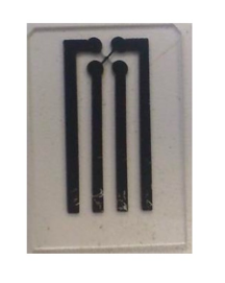
\includegraphics[]{sonda_test.pdf}\label{fig:sonda_test}}
    \subfloat[][]{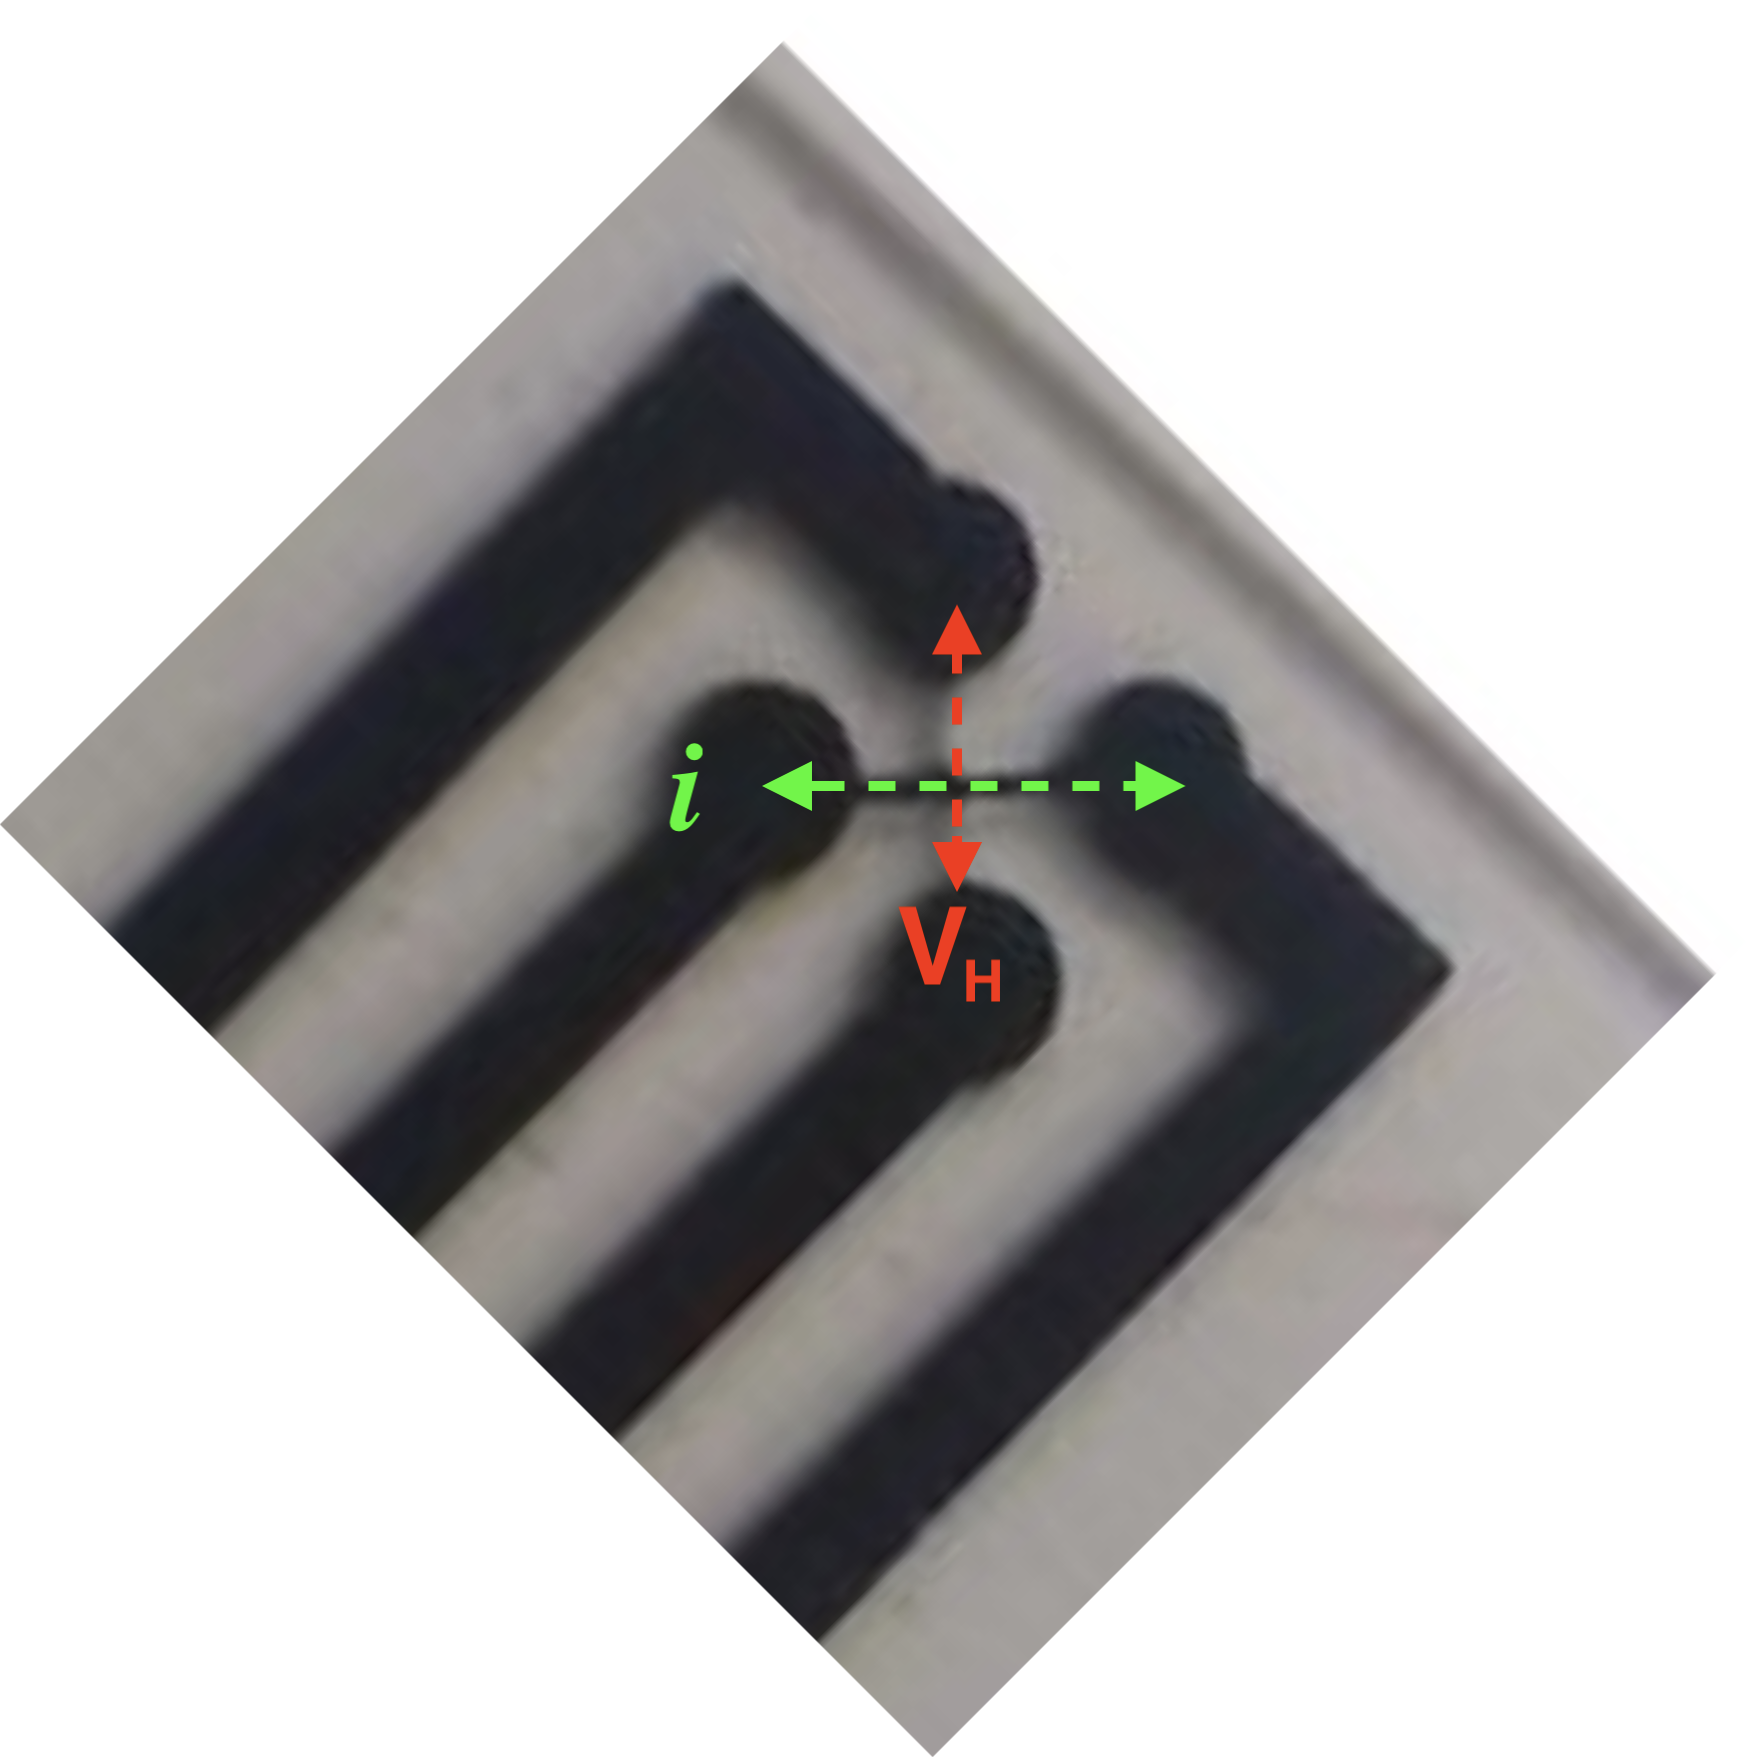
\includegraphics[width=0.25\linewidth]{zoomed_sonda.png}\label{fig:zoomed_sonda}}
    \caption{(a) Sonda utilizzata in laboratorio per la verifica dell'effetto Hall. (b) Ingrandimento ruotato di \SI{45}{\deg} della sonda sulla croce, ad indicare le direzioni di passaggio della corrente e di formazione della tensione di Hall $V_H$ (il campo magnetico è lungo la direzione ortogonale alla corrente $i$ e alla tensione $V_H$).}\label{fig:1}
\end{figure*}

\begin{table}
    \caption{(a) Dimensioni e caratteristiche della sonda utilizzata in laboratorio. (b) Alcune delle caratteristiche importanti delle strumentazioni utilizzate in laboratorio per l'esperienza. Il valore fixed value corrisponde ai casi in cui il valore della variabile non può essere cambiato, ed è limitato dalle condizioni di laboratorio (in generale indica i limiti entro cui possiamo scegliere il valore della variabile), Il valore avg. value corrisponde al valore che ricaviamo considerando sempre le limitazioni di laboratorio e che corrisponde alla miglior scelta che possiamo effettuare. Max STD indica il valore che possiamo stimare massimo per la deviazione standard sulla misura della variabile per avere una certa risoluzione sulla nostra misura (condizioni ottimali) in parti per mille.}
    \setcounter{table}{\numexpr\value{table}-1}
    \subfloat[][]{% \begin{ruledtabular}
    \begin{tabular}{lcc}
        \toprule
        MOD & Spessore $w$ (\si{\micro\metre}) & ERR (\si{\micro\metre})\\
        \colrule
        Sonda 2R & 3.3 & 0.2\\
        Sonda 6 & 12.2 & 0.6\\
        Sonda 1 & 8 & 0.5\\
        Sonda 3 & 3.8 & 0.2\\
        Sonda 2N & 6.1 & 0.3\\
        Sonda 4 & 4.5 & 0.2\\
        Sonda h5 & 3.6 & 0.2\\
        \toprule
    \end{tabular}
% \end{ruledtabular}\label{tab:sonda}}\hspace{5mm}
    \subfloat[][]{% \begin{ruledtabular}
    \begin{tabular}{lcccc}
        \toprule
        & fixed value & avg. value & max STD (ppt)\\
        \colrule
        Generatore elettrico ($i$) & - & \SI{10}{\milli\ampere} & - \\
        Campo magnetico $B$ & [0.1,0.5]\footnote{Massimo raggiungibile dagli strumenti di laboratorio, minimo importo per avere un effetto sostanzialmente utile (praticamente può andare fino a zero).} \si{\tesla} & - & - \\
        op-amp (per strum.) & - & $G\simeq 200$\footnote{Max. gain raggiungibile in condizioni di laboratorio?} & - \\
        \toprule
    \end{tabular}
% \end{ruledtabular}\label{tab:min_max_values}}
\end{table}

\end{document}